\documentclass[12pt]{article}
\usepackage[utf8]{inputenc}
\usepackage[spanish]{babel}
\usepackage{graphicx}
\usepackage{geometry}
\geometry{a4paper, margin=2.5cm}
\usepackage{titlesec}
\titleformat{\section}{\large\bfseries}{\thesection}{1em}{}

\title{An\'alisis Visual de la NBA 2025: Rendimiento Deportivo}
\author{}
\date{}

\begin{document}

\maketitle

\section*{Introducci\'on}

El presente informe tiene como objetivo analizar datos relevantes de la liga de baloncesto NBA correspondientes a la temporada 2025, utilizando herramientas de visualizaci\'on de datos. A partir de una amplia base estad\'istica, se pretende extraer conclusiones que expliquen el comportamiento competitivo de los equipos y su rendimiento a lo largo de la temporada. Para ello, se seleccion\'o como foco de estudio la dimensi\'on del \textbf{rendimiento deportivo}, por ser un aspecto clave y cuantificable mediante diversas m\'etricas disponibles en registros oficiales de la liga.

\section*{Elecci\'on de la 1 dimensi\'on: Rendimiento Deportivo}

La dimensi\'on seleccionada, \textbf{rendimiento deportivo}, permite evaluar cuantitativamente c\'omo se desempe\~naron los equipos dentro del marco competitivo. Esta dimensi\'on abarca tanto la producci\'on ofensiva como la eficacia general en el juego. De esta manera, se pueden identificar patrones de juego, fortalezas y debilidades entre los equipos, as\'i como el cumplimiento (o no) de sus expectativas seg\'un modelos estad\'isticos.

\section*{Criterio 1: Promedio de puntos por partido}

El primer criterio seleccionado fue el \textbf{promedio de puntos por partido} por equipo, una medida cl\'asica del rendimiento ofensivo. Se utiliz\'o un conjunto de datos oficiales de la NBA para representar esta m\'etrica mediante un \textit{violin plot}, el cual permite visualizar la distribuci\'on de los valores y la densidad en torno a la mediana. 

\begin{center}
    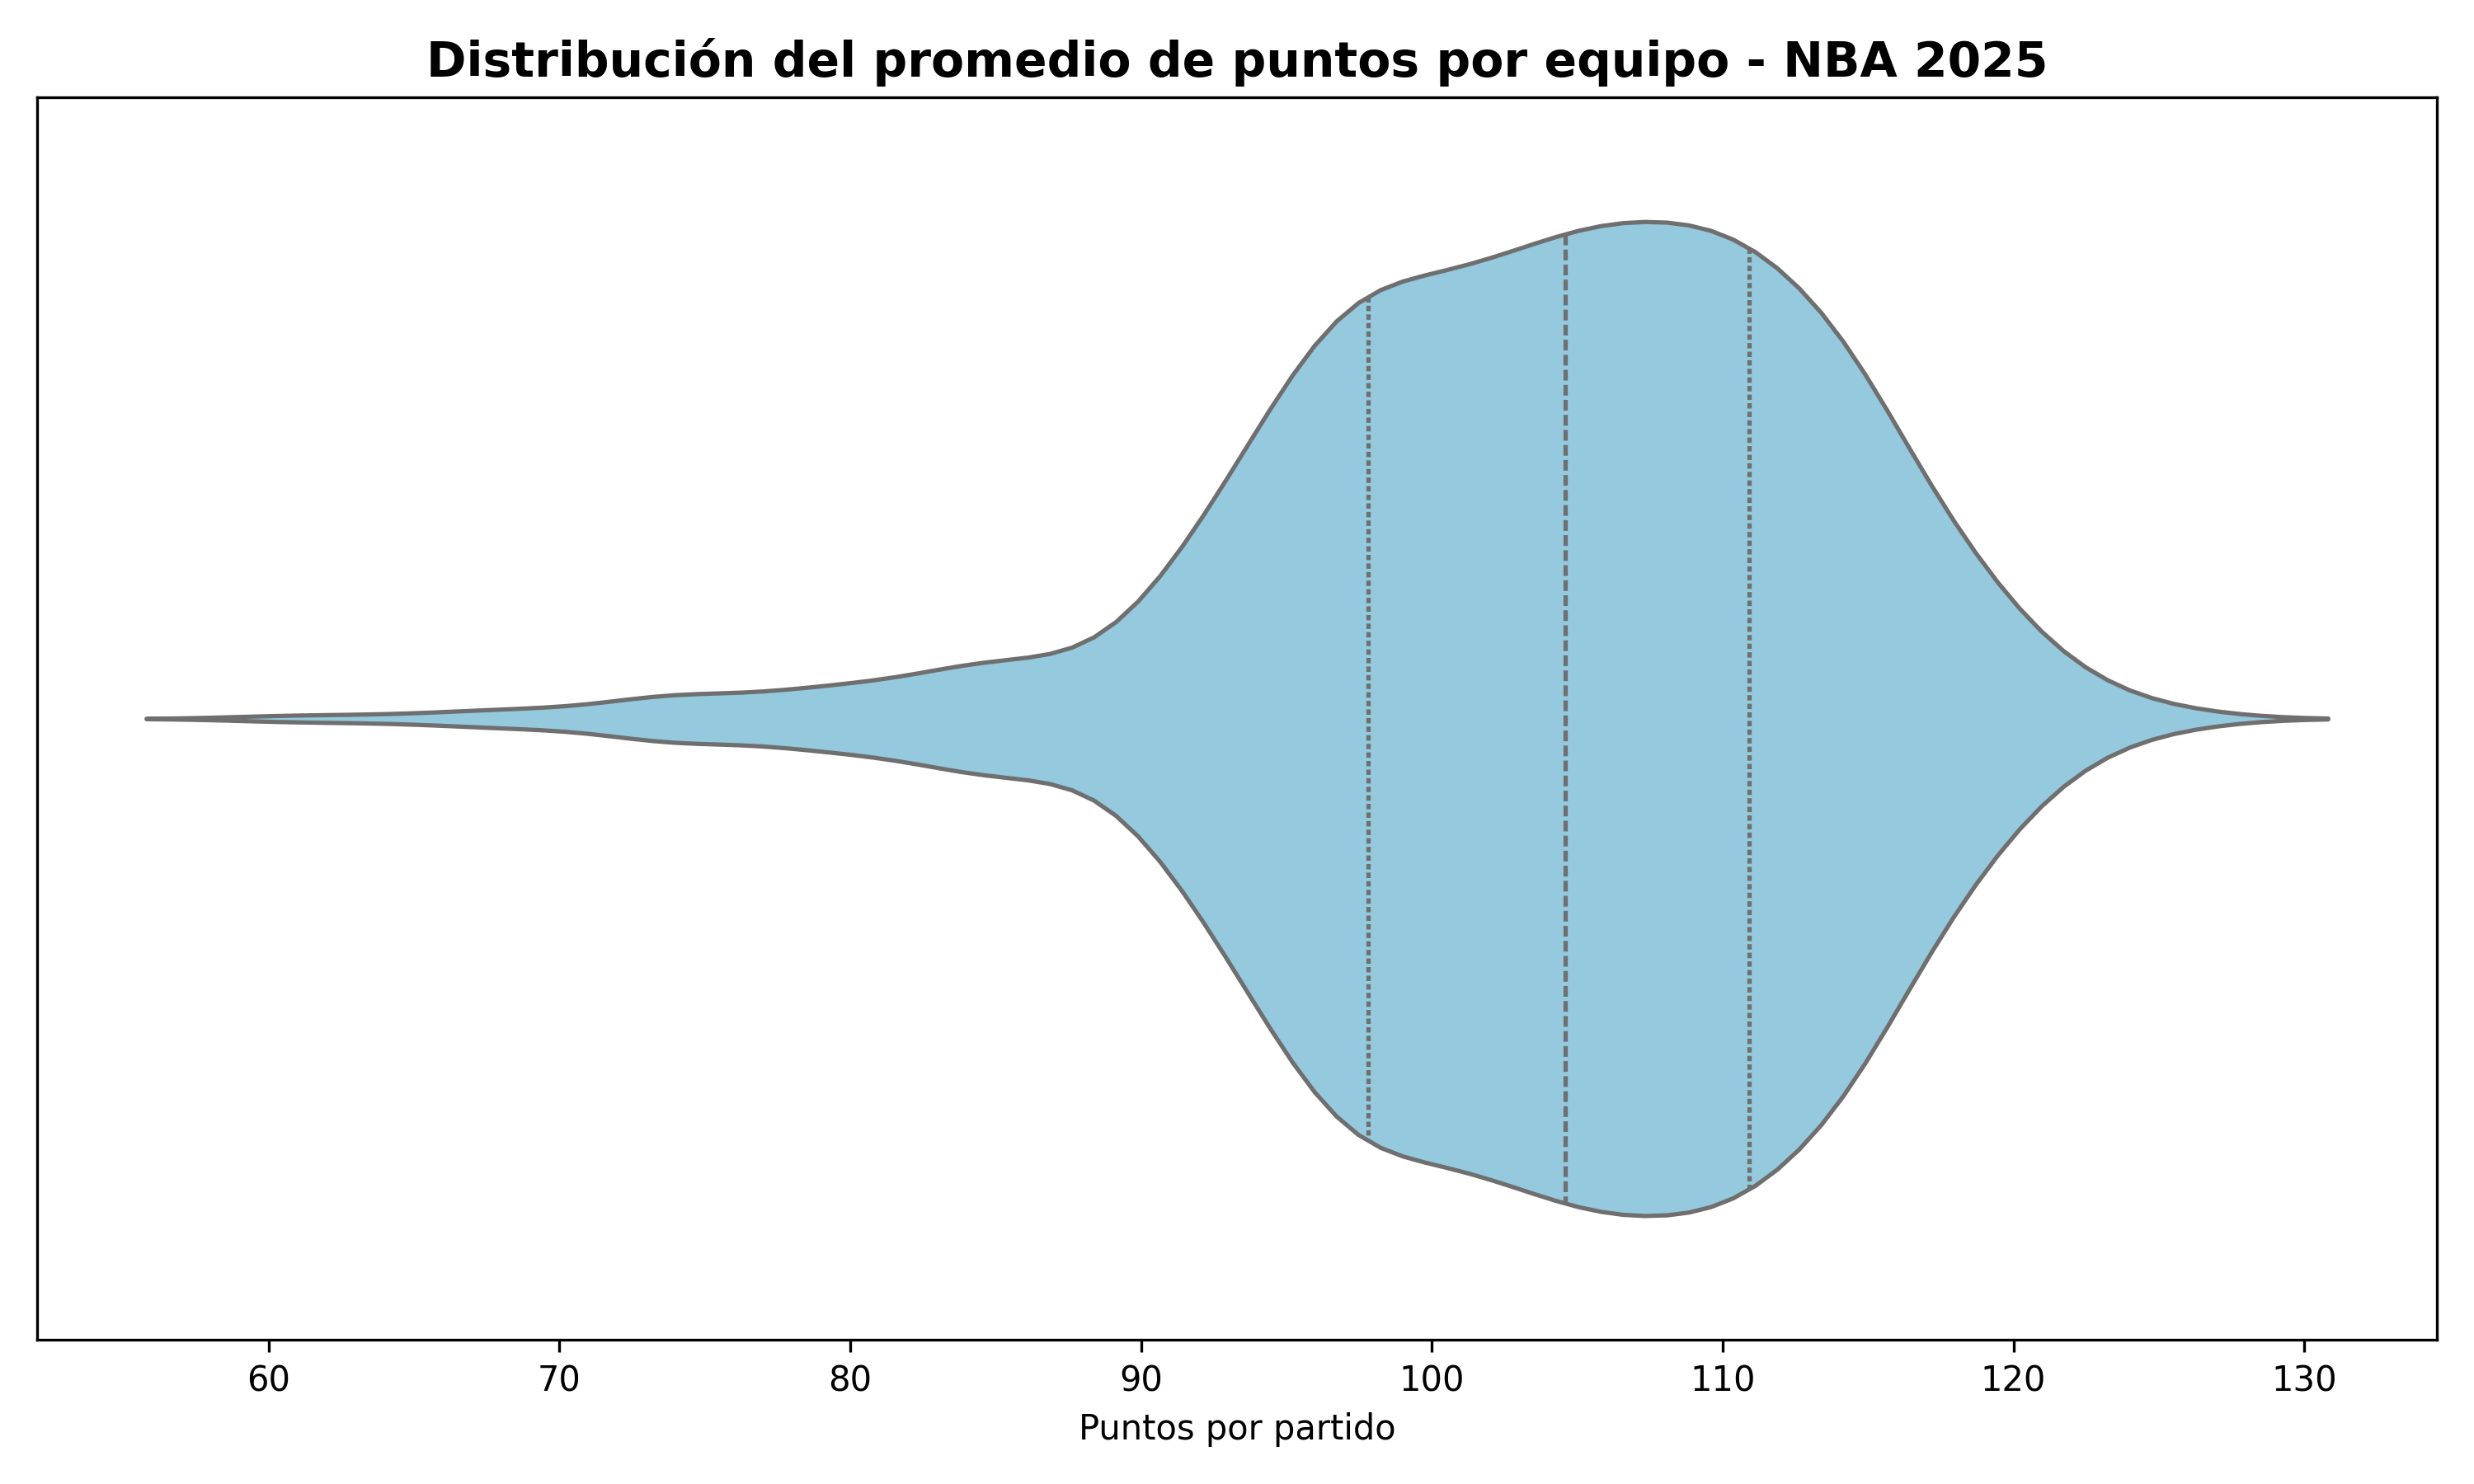
\includegraphics[width=0.7\textwidth]{violinplot_pts_per_game_nba2025.png}
\end{center}

\textbf{Conclusi\'on:} La mayor\'ia de los equipos anot\'o entre 105 y 115 puntos por partido, con algunos casos por debajo o por encima de este rango. Esto indica una relativa homogeneidad ofensiva, aunque tambi\'en permite identificar equipos con bajo poder anotador o con una ofensiva significativamente m\'as eficiente.

\section*{Criterio 2: Comparaci\'on entre victorias reales y esperadas}

El segundo criterio corresponde a la diferencia entre \textbf{victorias reales} y \textbf{victorias esperadas}, calculadas seg\'un modelos pythag\'oreos que utilizan los puntos anotados y recibidos. Para representar este criterio se utiliz\'o un \textit{Dumbbell Plot}, una visualizaci\'on no convencional que permite comparar visualmente ambos valores por equipo, destacando con claridad las discrepancias.

\begin{center}
    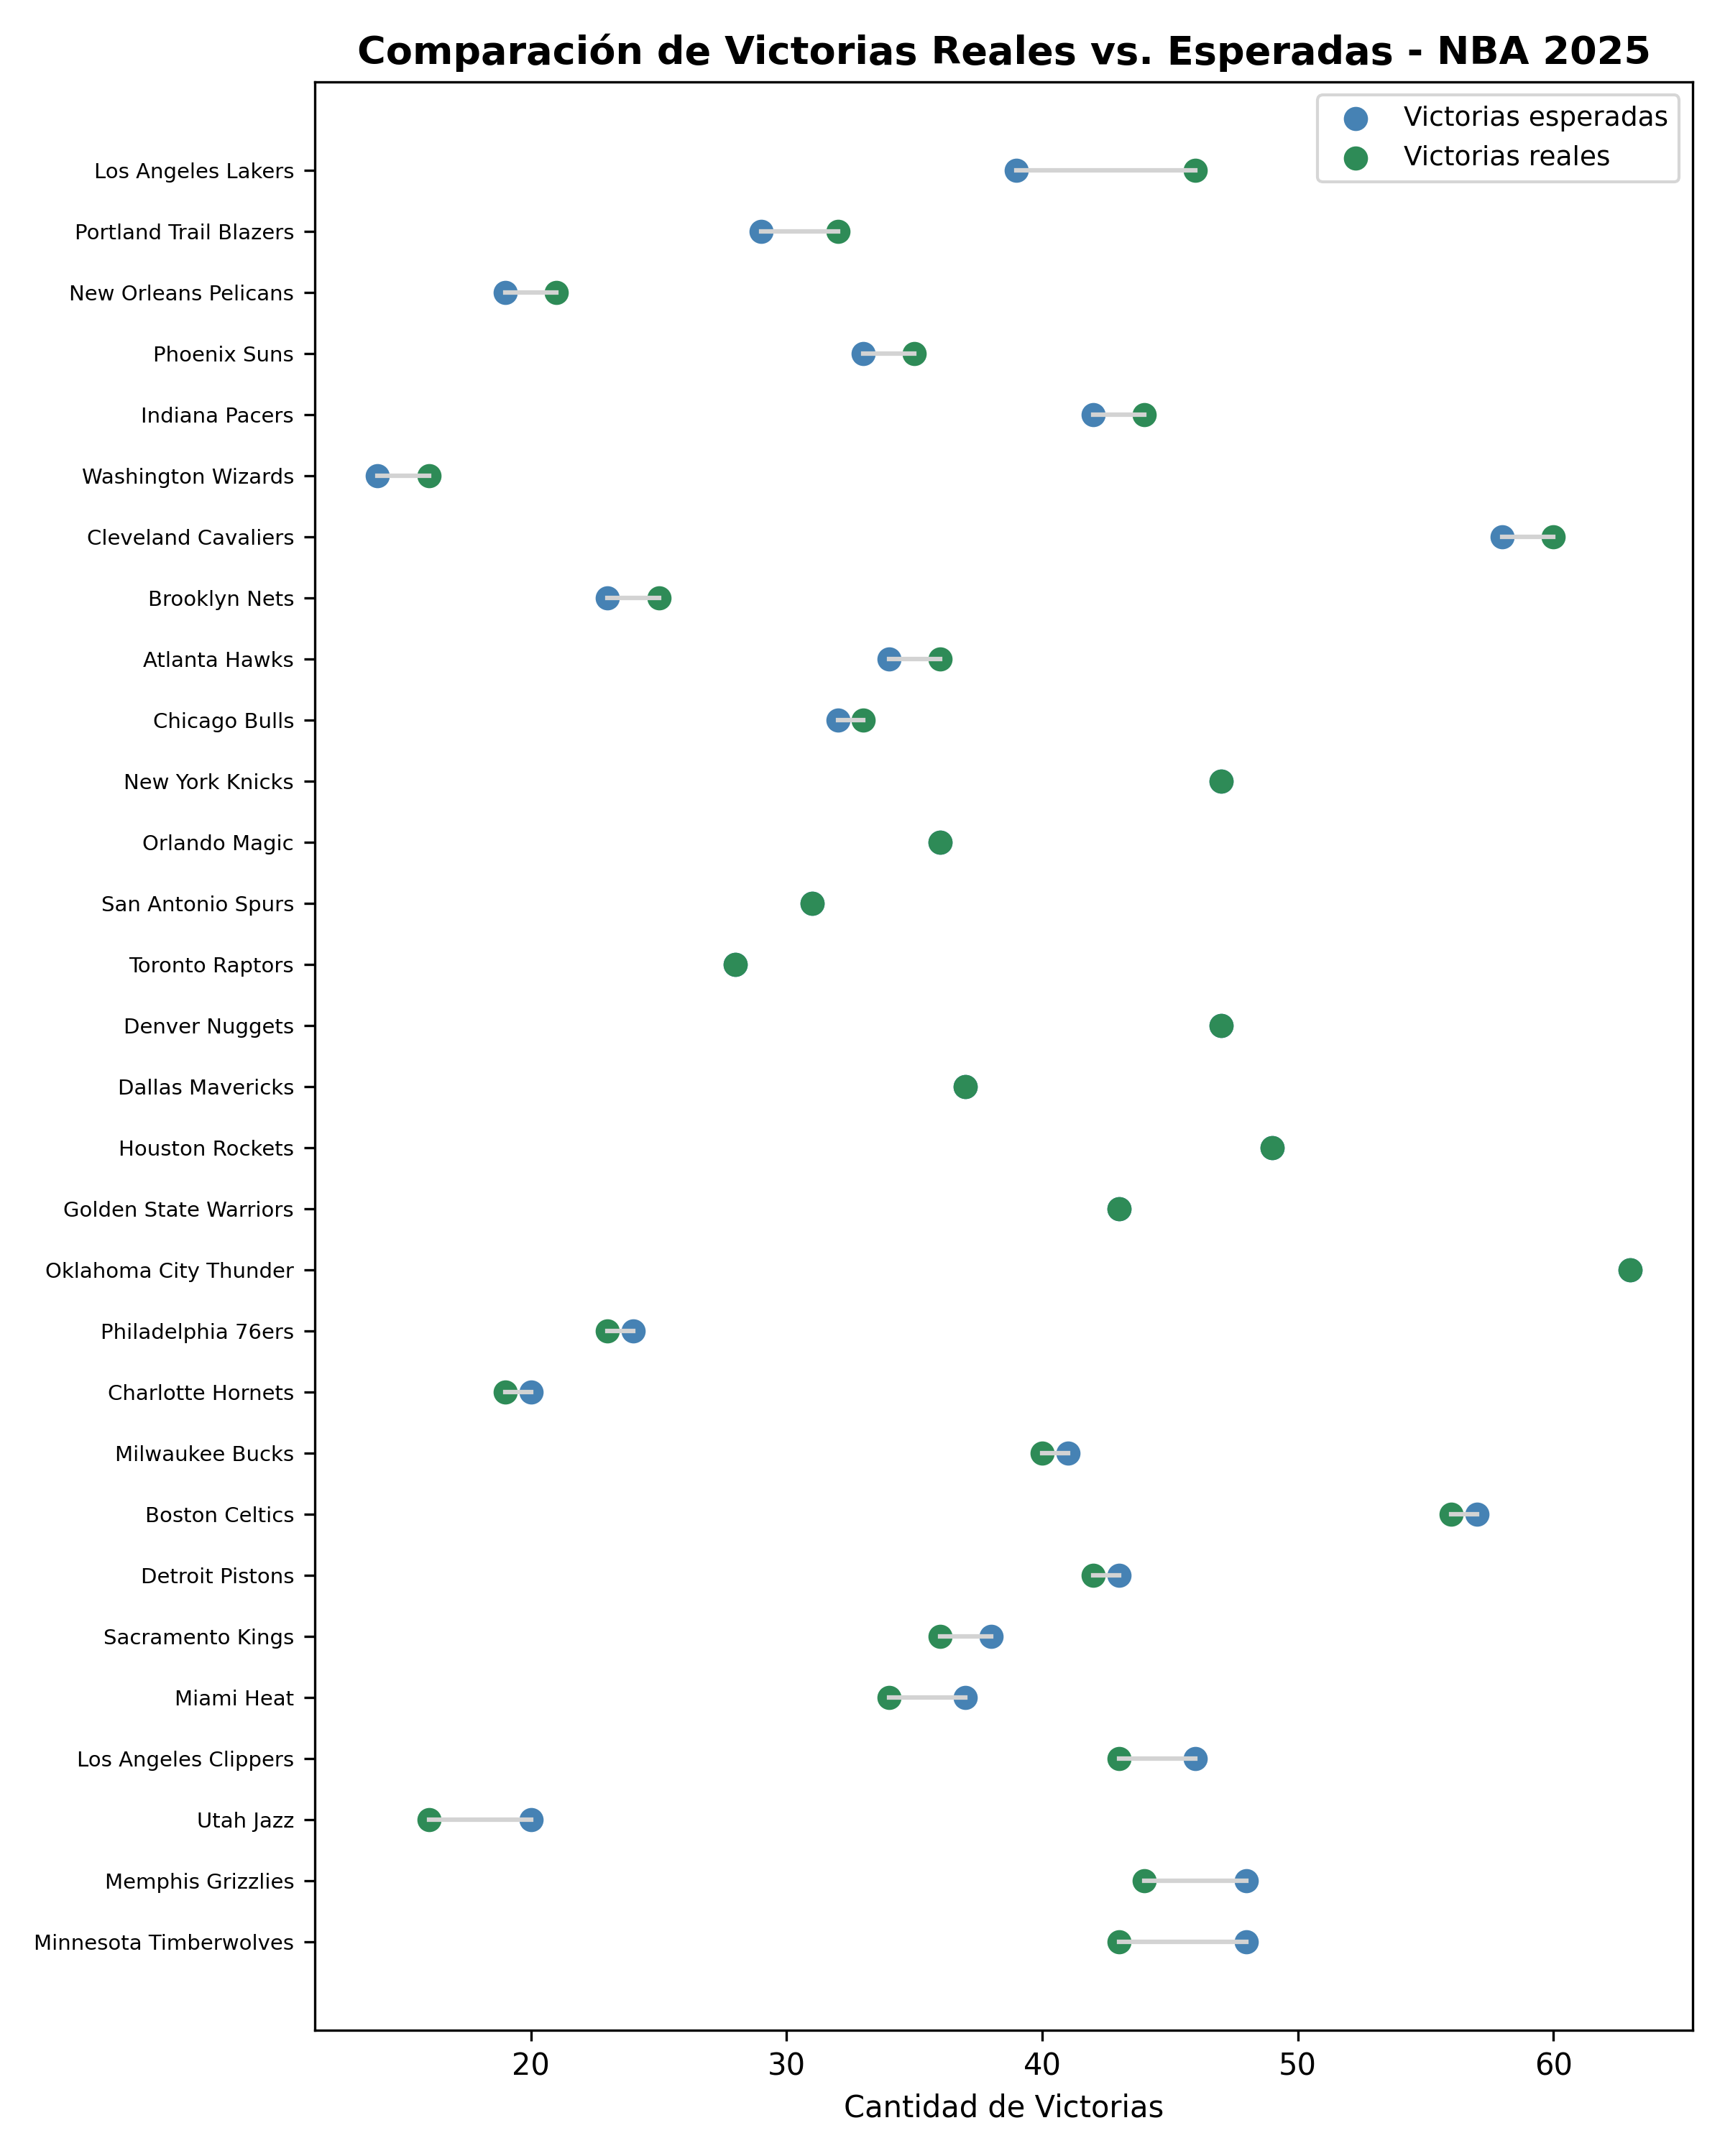
\includegraphics[width=0.8\textwidth]{dumbbell_plot_nba2025_victorias.png}
\end{center}

\textbf{Conclusi\'on:} Se observ\'o que varios equipos superaron las expectativas estad\'isticas, mientras que otros no alcanzaron su rendimiento proyectado. Las diferencias se atribuyen a factores como la ejecuci\'on en partidos cerrados, el rendimiento en momentos clave o incluso la suerte. El an\'alisis permite concluir que la estad\'istica esperada no siempre refleja el resultado final, pero ofrece una herramienta valiosa para evaluar eficiencia y consistencia competitiva.

\section*{Criterio 3: Relación entre pérdidas por posesión y derrotas}

Un indicador importante del rendimiento ofensivo de los equipos es la \textbf{tasa de pérdidas por posesión (TOV\%)}, que muestra cuántas veces un equipo pierde el balón antes de lanzar al aro. Para evaluar su impacto en los resultados, se comparó este porcentaje con la cantidad total de derrotas de cada equipo en la temporada 2025.

\begin{center}
    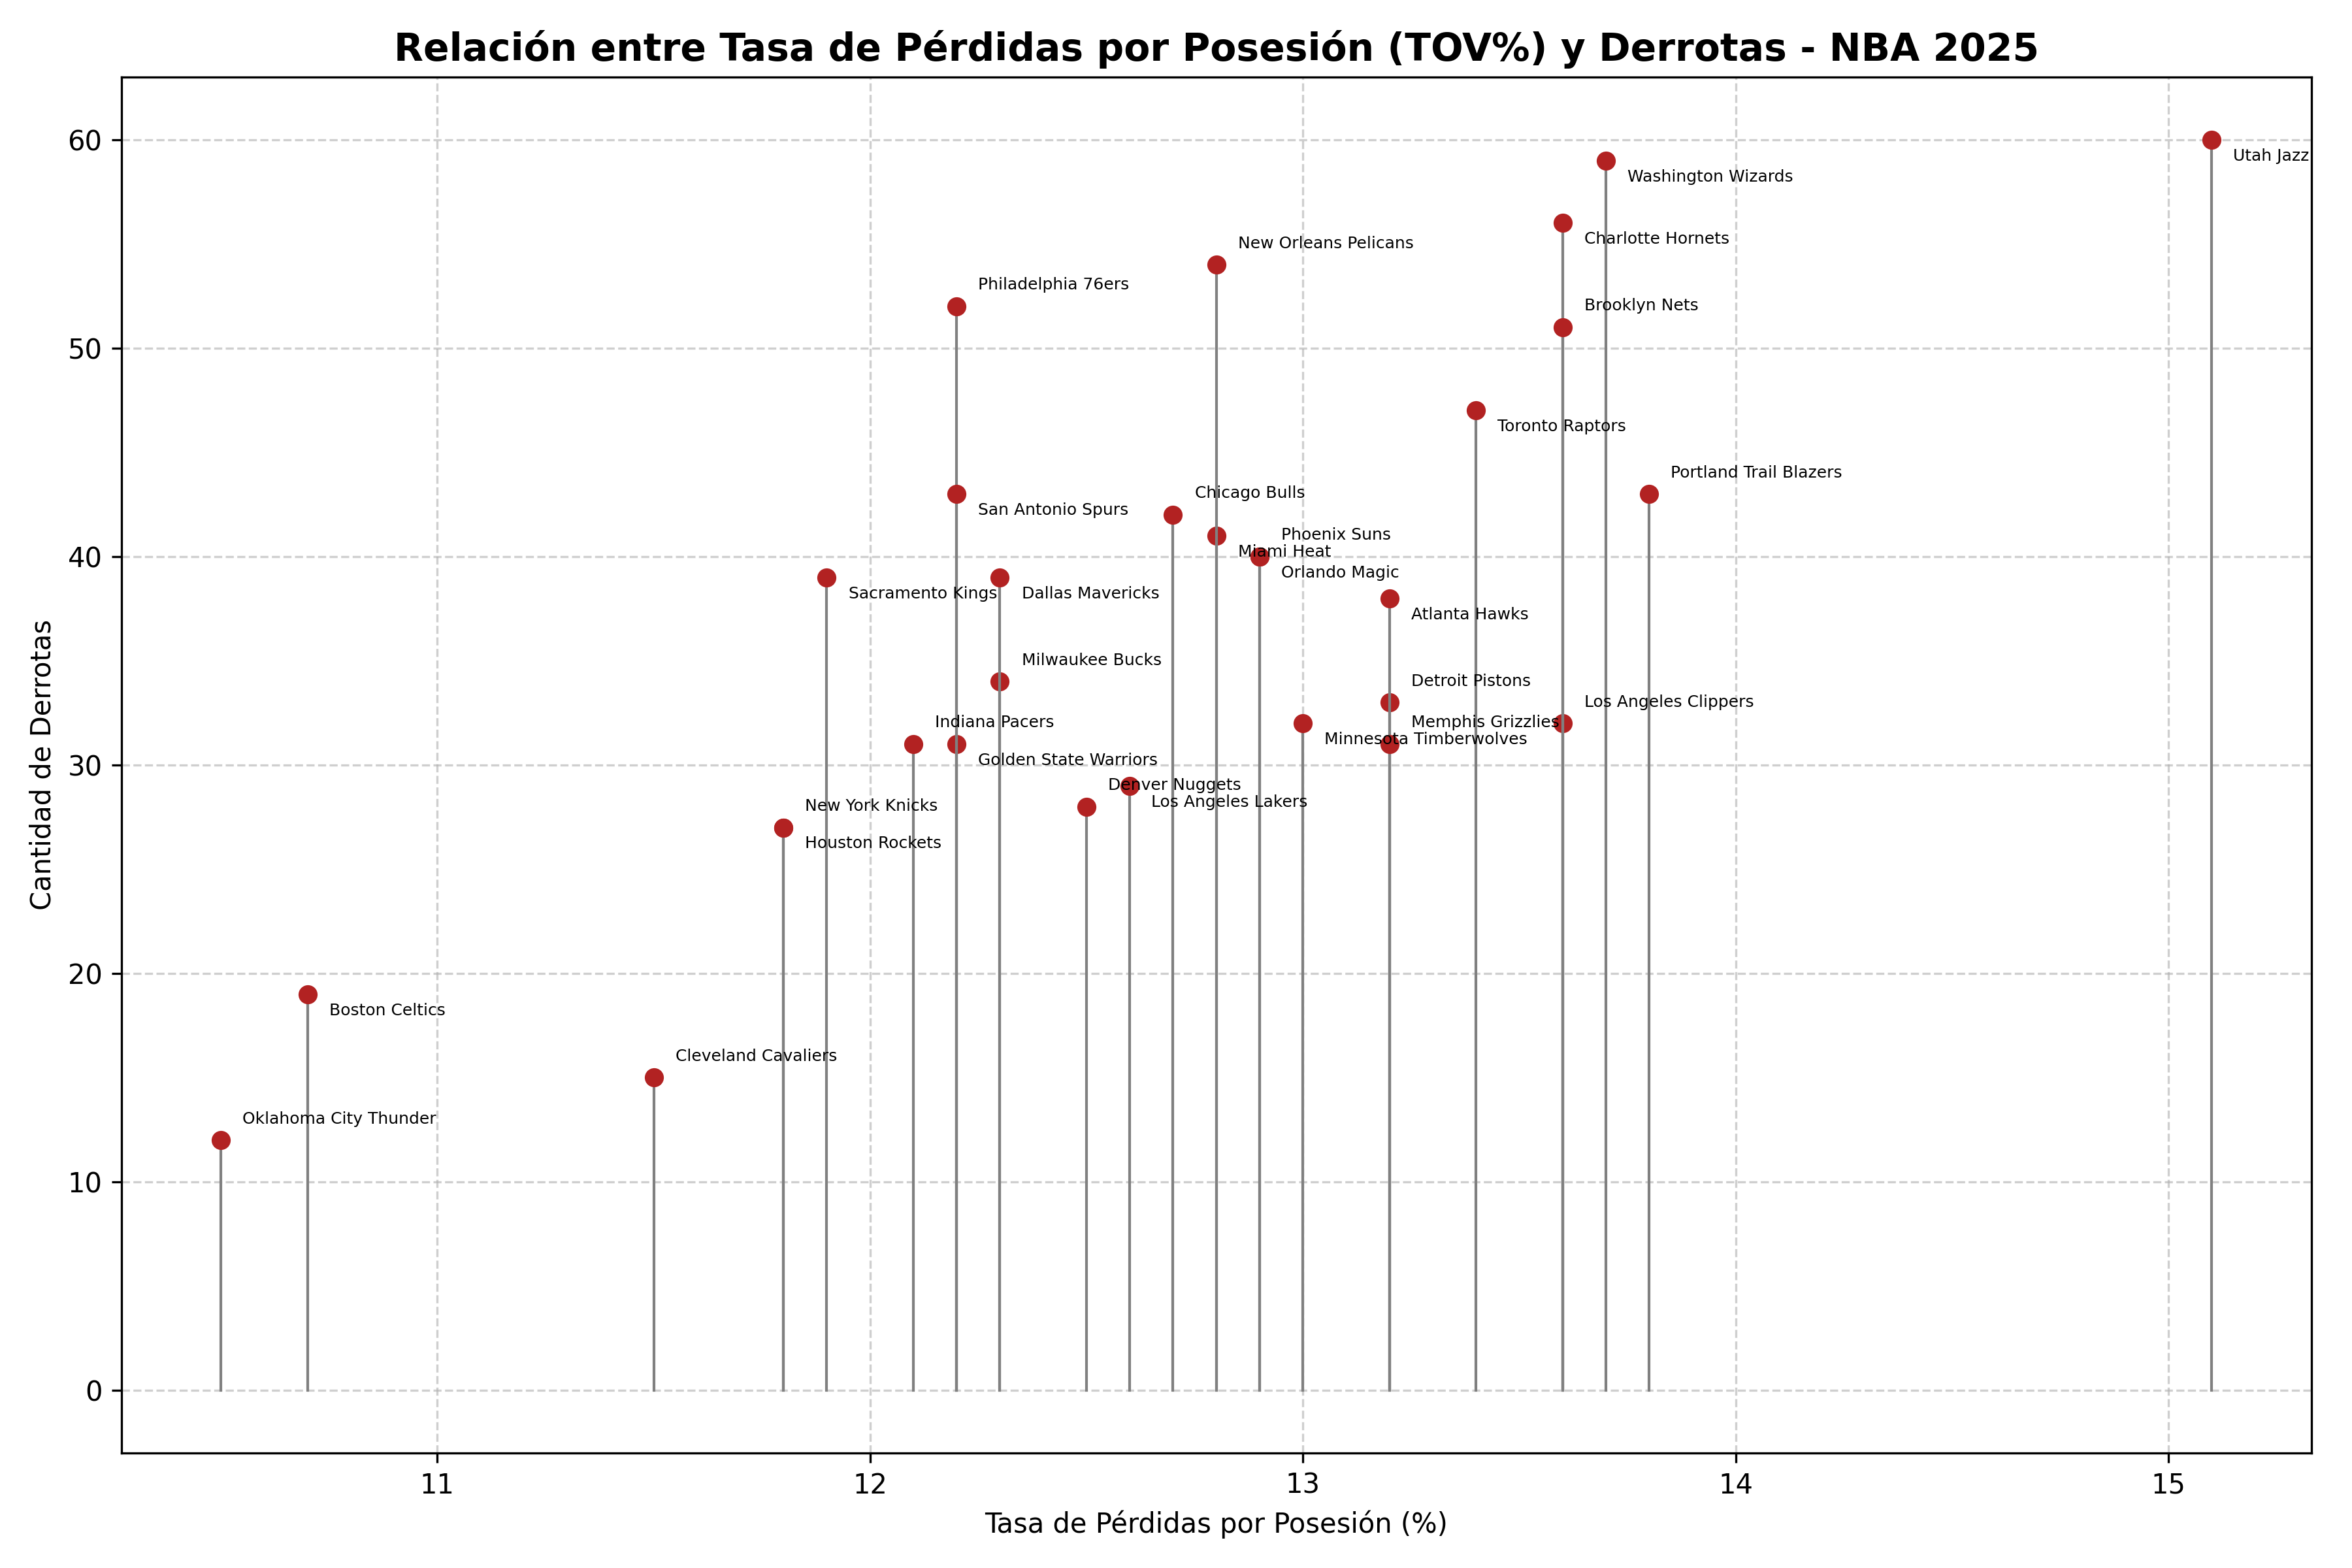
\includegraphics[width=0.8\textwidth]{lollipop_plot_tov_vs_derrotas.png}
\end{center}

\textbf{Conclusión:} El gráfico revela una tendencia clara: los equipos que registran una mayor proporción de pérdidas por posesión tienden a acumular más derrotas. Esto sugiere que el control del balón es un factor determinante en el desempeño competitivo. A pesar de algunas excepciones, la relación general valida que una ejecución ofensiva disciplinada influye directamente en el éxito durante la temporada.

\section*{Criterio 4: Distribución de Puntos por Partido según Posición y en distintos años.}

En la NBA, cada posición tiene roles distintos por lo que es un buen análisis como se distribuyen los puntos según, en este caso, en temporadas muy alejadas. Se pueden observar como ha cambiado la forma del juego con los años debido a transformaciones tácticas, mayor ritmo de juego, incorporación de lanzamientos de triple, entre otros factores.


\begin{center}
    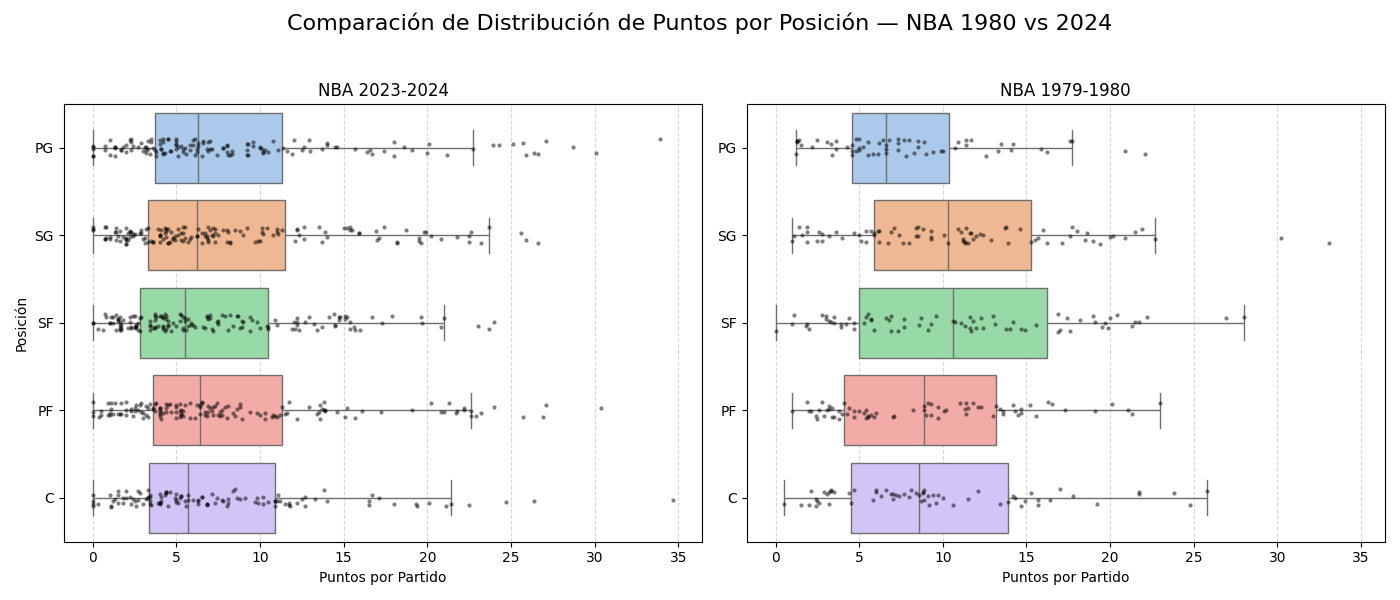
\includegraphics[width=0.8\textwidth]{boxplot.png}
\end{center}

\textbf{Conclusión:} Se observó como el protagonismo de los puntos cambia totalmente, se pasa de un juego con mayor protagonismo de los Escoltas (SG) y Aleros (SF) en 1980, a una distribución mucho más pareja en 2024. También se observa un aumento en la cantidad total de puntos con los años y que pocos jugadores en 1980 alcanzaban un promedio de +25 puntos con respecto al año 2024.


\end{document}
